\documentclass[8pt,a4paper,compress]{beamer}

\usepackage{/home/siyer/lib/slides}

\title{Tries}
\date{}
\begin{document}
\begin{frame}
\vfill
\titlepage
\end{frame}

\begin{frame}
\frametitle{Outline}
\tableofcontents
\end{frame}

\section{Tries}
\begin{frame}[fragile]
\pause

API for a symbol table with string keys
\begin{center}
\begin{tabular}{cc}
method & description \\ \hline
\lstinline$StringST()$ & create a symbol table \\ 
\lstinline$Value get(String key)$ & value paired with key (\lstinline$null$ if $key$ is absent) \\
\lstinline$boolean contains(String key)$ & is there a value paired with $key$? \\
\lstinline$void put(String key, Value val)$ & \makecell{put key-value pair into the table \\ (remove $key$ if value is \lstinline$null$)} \\
\lstinline$int size()$ & number of key-value pairs \\
\lstinline$boolean isEmpty()$ & is the table empty? \\
\lstinline$Iterable<String> keys()$ & all the keys in the table \\
\lstinline$Iterable<String> keysWithPrefix(String s)$ & all the keys having $s$ as a prefix \\
\lstinline$Iterable<String> keysThatMatch(String s)$ & \makecell{all the keys that match $s$ \\ (where \lstinline$.$ matches any character)} \\
\lstinline$String longestPrefixOf(String s)$ & the longest key that is a prefix of $s$ \\
\lstinline$void delete(String key)$ & remove $key$ (and its value) \\
\end{tabular}
\end{center}
\end{frame}

\begin{frame}[fragile]
\begin{minipage}{160pt}
\pause

A trie is a search tree data structure built from the characters of string keys that allows us to use the characters of the search key to guide the search

\pause
\bigskip

Tries are composed of nodes that contain links that are either null or references to other nodes

\pause
\bigskip

Each node is pointed to by just one other node, which is called its parent (except for one node, the root, which has no nodes pointing to it), and each node has $R$ links, where $R$ is the alphabet size

\pause
\bigskip

Each node also has a corresponding value, which may be null or the value associated with one of the string keys in the symbol table

\pause
\bigskip

Nodes with null values exist to facilitate search in the trie and do
not correspond to keys
\end{minipage}\hfill %
\begin{minipage}{140pt}
\begin{center}
\visible<2->{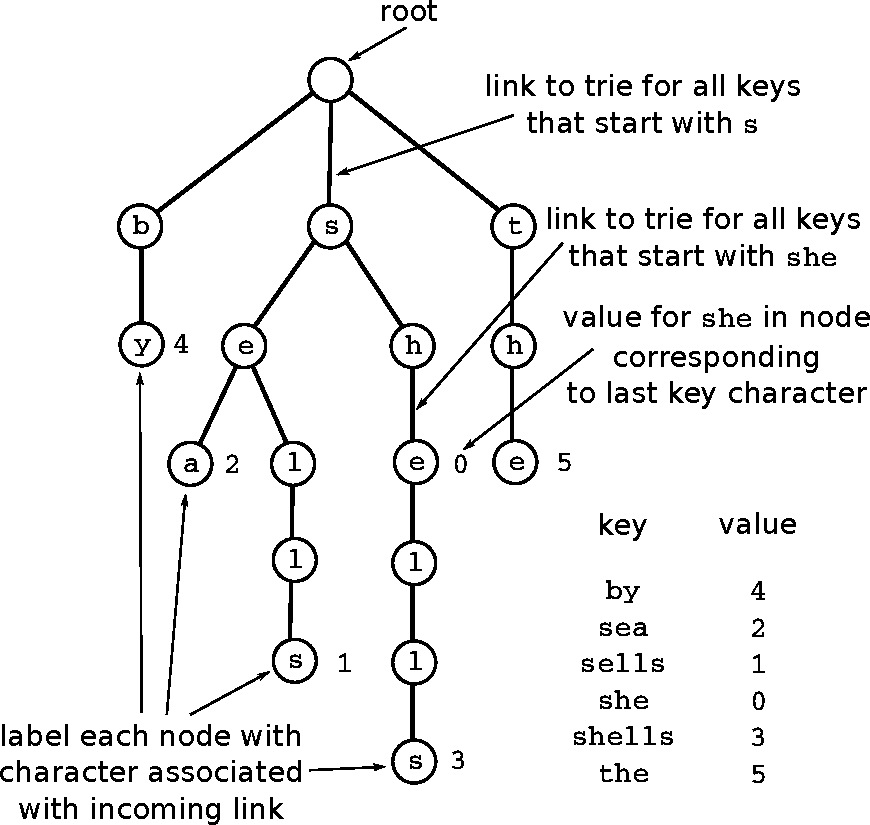
\includegraphics[scale=0.35]{{./figures/trie1}.pdf}}
\end{center}
\end{minipage}
\end{frame}

\begin{frame}[fragile]
\pause

Search in a trie

\begin{center}
\visible<2->{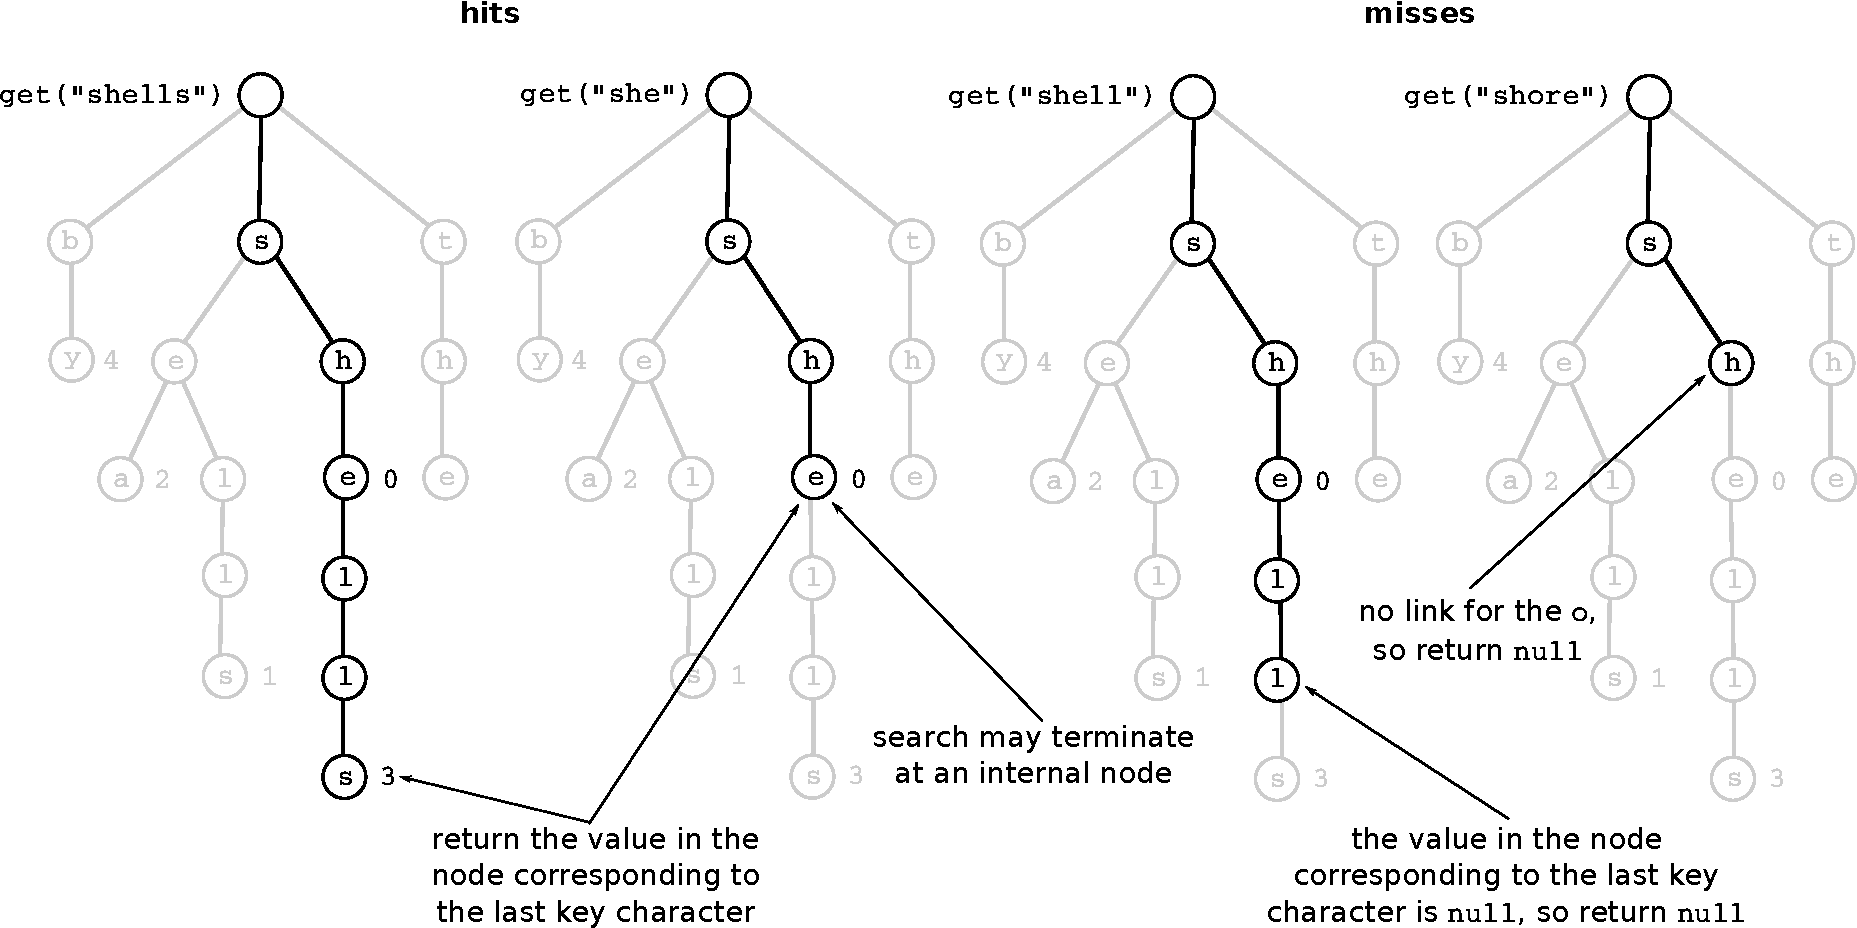
\includegraphics[scale=0.35]{{./figures/trie2}.pdf}}
\end{center}
\end{frame}

\begin{frame}[fragile]
\pause

Insertion into a trie

\begin{center}
\visible<2->{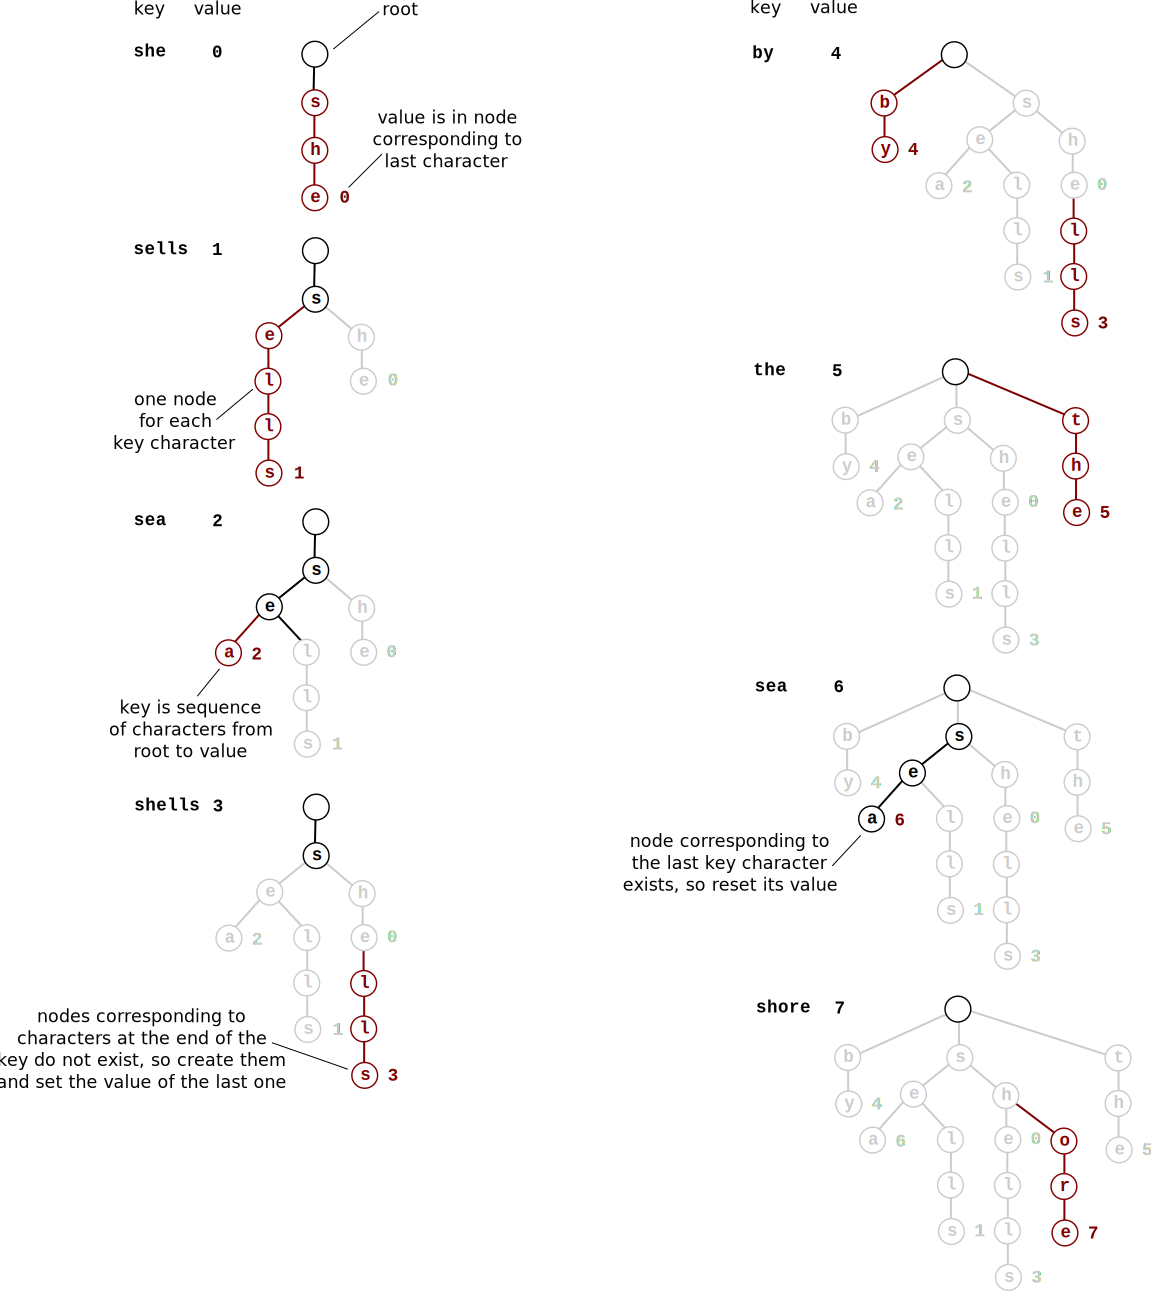
\includegraphics[scale=0.23]{{./figures/trie3}.pdf}}
\end{center}
\end{frame}

\begin{frame}[fragile]
\pause

Deletion

\begin{center}
\visible<2->{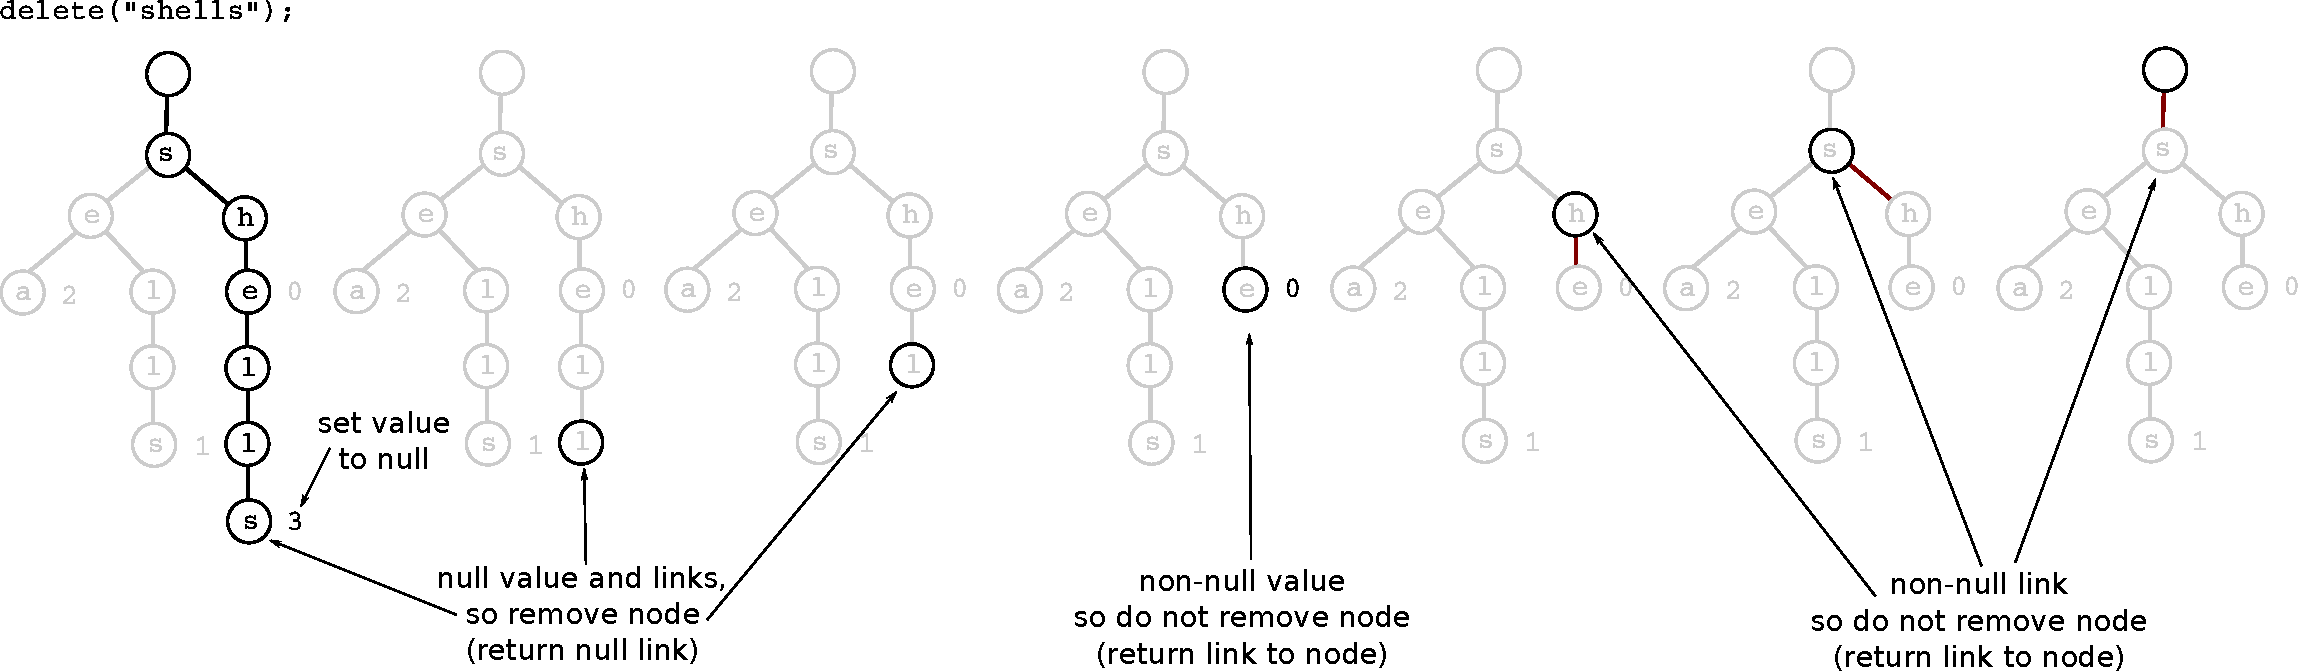
\includegraphics[scale=0.28]{{./figures/trie4}.pdf}}
\end{center}
\end{frame}

\begin{frame}[fragile]
\pause

Trie representation ($R = 26$)

\begin{center}
\visible<2->{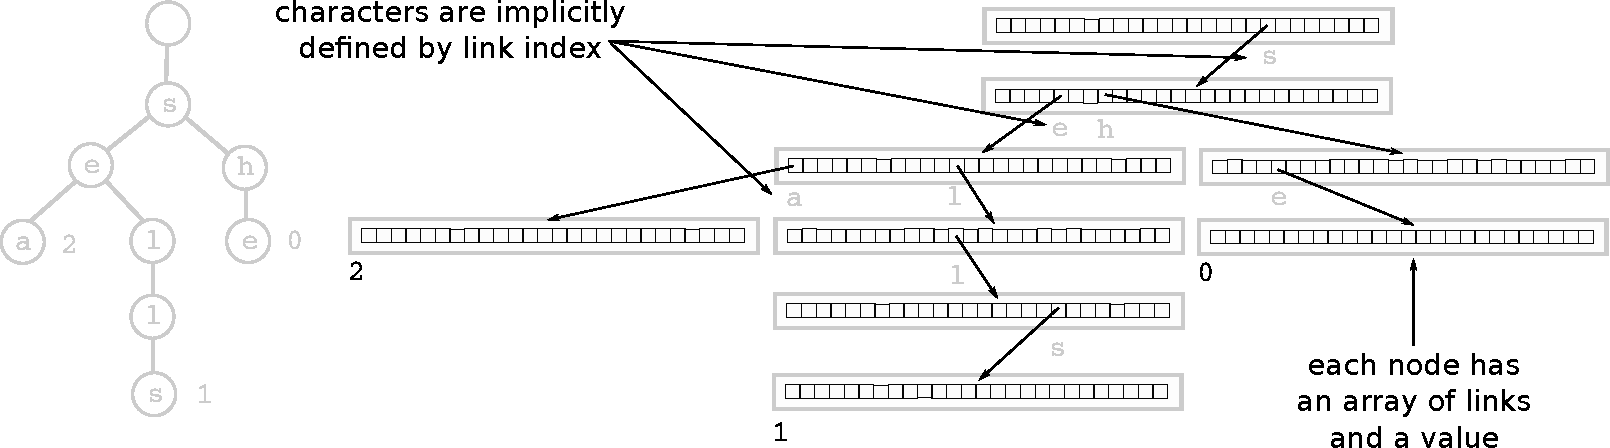
\includegraphics[scale=0.4]{{./figures/trie5}.pdf}}
\end{center}
\end{frame}

\begin{frame}[fragile]
\pause

\begin{lstlisting}[language=Java]
package edu.princeton.cs.algs4;

public class TrieST<Value> {
    private static final int R = 256;
    private Node root; 
    private int N; 

    private static class Node {
        private Object val;
        private Node[] next = new Node[R];
    }

    public TrieST() { }

    public Value get(String key) {
        Node x = get(root, key, 0);
        if (x == null) { return null; }
        return (Value) x.val;
    }

    private Node get(Node x, String key, int d) {
        if (x == null) { return null; }
        if (d == key.length()) { return x; }
        char c = key.charAt(d);
        return get(x.next[c], key, d + 1);
    }

    public boolean contains(String key) { return get(key) != null; }

    public void put(String key, Value val) {
        if (val == null) { delete(key); }
        else { root = put(root, key, val, 0); }
    }
\end{lstlisting}
\end{frame}

\begin{frame}[fragile]
\pause

\begin{lstlisting}[language=Java]
    private Node put(Node x, String key, Value val, int d) {
        if (x == null) { x = new Node(); }
        if (d == key.length()) {
            if (x.val == null) { N++; }
            x.val = val;
            return x;
        }
        char c = key.charAt(d);
        x.next[c] = put(x.next[c], key, val, d + 1);
        return x;
    }

    public int size() { return N; }

    public boolean isEmpty() { return size() == 0; }

    public Iterable<String> keys() { return keysWithPrefix(""); }

    public Iterable<String> keysWithPrefix(String prefix) {
        LinkedQueue<String> results = new LinkedQueue<String>();
        Node x = get(root, prefix, 0);
        collect(x, new StringBuilder(prefix), results);
        return results;
    }

    private void collect(Node x, StringBuilder prefix, 
                         LinkedQueue<String> results) {
        if (x == null) { return; }
        if (x.val != null) { results.enqueue(prefix.toString()); }
        for (char c = 0; c < R; c++) {
            prefix.append(c);
            collect(x.next[c], prefix, results);
            prefix.deleteCharAt(prefix.length() - 1);
        }
    }
\end{lstlisting}
\end{frame}

\begin{frame}[fragile]
\pause

\begin{lstlisting}[language=Java]
    public Iterable<String> keysThatMatch(String pattern) {
        LinkedQueue<String> results = new LinkedQueue<String>();
        collect(root, new StringBuilder(), pattern, results);
        return results;
    }

    private void collect(Node x, StringBuilder prefix, String pattern, 
                         LinkedQueue<String> results) {
        if (x == null) { return; }
        int d = prefix.length();
        if (d == pattern.length() && x.val != null) {
            results.enqueue(prefix.toString());
        }
        if (d == pattern.length()) { return; }
        char c = pattern.charAt(d);
        if (c == '.') {
            for (char ch = 0; ch < R; ch++) {
                prefix.append(ch);
                collect(x.next[ch], prefix, pattern, results);
                prefix.deleteCharAt(prefix.length() - 1);
            }
        }
        else {
            prefix.append(c);
            collect(x.next[c], prefix, pattern, results);
            prefix.deleteCharAt(prefix.length() - 1);
        }
    }

    public String longestPrefixOf(String query) {
        int length = longestPrefixOf(root, query, 0, -1);
        if (length == -1) { return null; }
        return query.substring(0, length); 
    }
\end{lstlisting}
\end{frame}

\begin{frame}[fragile]
\pause

\begin{lstlisting}[language=Java]
    private int longestPrefixOf(Node x, String query, int d, int length) {
        if (x == null) { return length; }
        if (x.val != null) { length = d; }
        if (d == query.length()) { return length; }
        char c = query.charAt(d);
        return longestPrefixOf(x.next[c], query, d + 1, length);
    }

    public void delete(String key) { root = delete(root, key, 0); }

    private Node delete(Node x, String key, int d) {
        if (x == null) { return null; }
        if (d == key.length()) {
            if (x.val != null) { N--; }
            x.val = null;
        }
        else {
            char c = key.charAt(d);
            x.next[c] = delete(x.next[c], key, d + 1);
        }
        if (x.val != null) { return x; }
        for (int c = 0; c < R; c++) {
            if (x.next[c] != null) { return x; }
        }
        return null;
    }
\end{lstlisting}
\end{frame}

\begin{frame}[fragile]
\pause

\begin{lstlisting}[language=Java]
    public static void main(String[] args) {
        TrieST<Integer> st = new TrieST<Integer>();
        for (int i = 0; !StdIn.isEmpty(); i++) {
            String key = StdIn.readString();
            st.put(key, i);
        }
        if (st.size() < 100) {
            StdOut.println("keys(\"\"):");
            for (String key : st.keys()) {
                StdOut.println(key + " " + st.get(key));
            }
            StdOut.println();
        }
        StdOut.println("longestPrefixOf(\"shellsort\"):");
        StdOut.println(st.longestPrefixOf("shellsort"));
        StdOut.println();
        StdOut.println("longestPrefixOf(\"quicksort\"):");
        StdOut.println(st.longestPrefixOf("quicksort"));
        StdOut.println();
        StdOut.println("keysWithPrefix(\"shor\"):");
        for (String s : st.keysWithPrefix("shor")) { 
            StdOut.println(s); 
        }
        StdOut.println();
        StdOut.println("keysThatMatch(\".he.l.\"):");
        for (String s : st.keysThatMatch(".he.l.")) { 
            StdOut.println(s); 
        }
    }
}
\end{lstlisting}
\end{frame}

\begin{frame}[fragile]
\pause

\begin{lstlisting}[language={}]
$ more shellsST.txt 
she sells sea shells by the sea shore
\end{lstlisting}

\pause

\begin{lstlisting}[language={}]
$ java edu.princeton.cs.algs4.TrieST < shellsST.txt 
keys(""):
by 4
sea 6
sells 1
she 0
shells 3
shore 7
the 5

longestPrefixOf("shellsort"):
shells

longestPrefixOf("quicksort"):
null

keysWithPrefix("shor"):
shore

keysThatMatch(".he.l."):
shells
\end{lstlisting}
\end{frame}

\section{Properties of Tries}
\begin{frame}[fragile]
\pause

The linked structure (shape) of a trie is independent of the key insertion/deletion order: there is a unique trie for any given set of keys

\pause
\bigskip

The number of array accesses when searching in a trie or inserting
a key into a trie is at most 1 plus the length of the key

\pause
\bigskip

The average number of nodes examined for search miss in a trie built from $N$ random keys over an alphabet of size $R$ is $\sim \log_R N$

\pause
\bigskip

The number of links in a trie is between $RN$ and $RNw$, where $w$ is
the average key length
\end{frame}


\section{Performance Characteristics of String-searching Algorithms}
\begin{frame}[fragile]
\pause

\begin{center}
\begin{tabular}{cccc}
\makecell{algorithm \\ (data structure)} & \makecell{characters \\ examined for \\ search miss} & memory usage & sweet spot \\ \hline
\makecell{binary tree search \\ (BST)} & $c_1(\lg N)^2$ & $64N$ & \makecell{randomly ordered \\ keys} \\
\makecell{2-3 tree search \\ (red-black BST)} & $c_2(\lg N)^2$ & $64N$ & \makecell{guaranteed performance} \\
\makecell{trie search \\ ($R$-way trie)} & $\log_R N$ & \makecell{$(8R + 56)N$ to \\ $(8R+56)Nw$} & \makecell{short keys \\ small alphabets} \\
\makecell{trie search \\ (ternary search trie (TST))} & $1.39\lg N$ & $64N$ to $64Nw$ & nonrandom keys
\end{tabular}

\bigskip

$\dagger \ddagger$ Typical growth rate for $N$ strings from an $R$-character alphabet (average length $w$)
\end{center}
\end{frame}
\end{document}
